
\documentclass[10pt,answers]{exam}
\usepackage[left=20mm,top=25mm,right=20mm,bottom=18mm]{geometry}
%\usepackage[a4paper,left=20mm,right=20mm]{geometry}
\usepackage{etex}
\usepackage{amssymb,amsmath,multicol} %<-- InWorksheetExam1 i also have fancyhdr,

\usepackage[metapost]{mfpic}
\usepackage[pdftex]{graphicx}

\usepackage{pst-plot}
\usepackage{pgfplots}
\pgfplotsset{compat=1.9}

\usepackage{tikz}
\usepackage{tkz-2d}
\usepackage{tkz-base}
\usetikzlibrary{calc}
\usepackage{tabu}
\usepackage{systeme}
\usepgfplotslibrary{fillbetween}

\usepackage[inline]{enumitem}
\usepackage{refcount}%<-- non in WorksheetExam1

\usepackage{caption}

\usepackage{array}
\newcolumntype{L}[1]{>{\raggedright\let\newline\\\arraybackslash\hspace{0pt}}m{#1}}
\newcolumntype{C}[1]{>{\centering\let\newline\\\arraybackslash\hspace{0pt}}m{#1}}
\newcolumntype{R}[1]{>{\raggedleft\let\newline\\\arraybackslash\hspace{0pt}}m{#1}}

%\renewcommand{\headrulewidth}{0pt}

\newcommand{\vasymptote}[2][]{
    \draw [densely dashed,#1] ({rel axis cs:0,0} -| {axis cs:#2,0}) -- ({rel axis cs:0,1} -| {axis cs:#2,0});
}

%%%%\renewcommand\partlabel{(\thequestion.\arabic{partno})}




%--------------------------------------------------------------------
\newcounter{numpofq}

% The argument to \numpartsofquestion should be an arabic number that
% is the number of a question.  We set the counter numpofq to the
% number of parts of question number argument.
\newcommand{\setcountertopartsofq}[1]{%
	\def\qnotemp{#1}%
	\setcounter{numpofq}{1}%
	% We go to \numpofqrelay to increment numpofq until we find
	% a part number that doesn't exist:
	\numpofqrelay
}% setcountertopartsofq

\def\numpofqrelay{%
	\expandafter\ifx\csname Pg@part@\qnotemp
	@\arabic{numpofq}\endcsname\relax
	% This part number doesn't exist; back up one and exit:
	\addtocounter{numpofq}{-1}%
	\let\nextnumpofqrelay=\relax
	\else
	% This part number exists; try the next number:
	\addtocounter{numpofq}{1}%
	\let\nextnumpofqrelay=\numpofqrelay
	\fi
	\nextnumpofqrelay
}% numpofqrelay

\makeatletter
\def\wordnum#1{\expandafter\word\csname c@#1\endcsname}
\def\word#1{%
	\ifcase #1 zero\or one\or two\or three\or four\or five\or six\or
	seven\or eight\or nine\or ten\or eleven\or twelve\or thirteen\or
	fourteen\or fifteen\or sixteen\or seventeen\or eighteen\or
	nineteen\or twenty\else too many\fi
}% word
\makeatother
%------------------------------------




\addpoints
%\printanswers
\noprintanswers

\opengraphsfile{Exam1B_Fa18}

\begin{document}
\extrawidth{-0.3in}
\pagestyle{headandfoot}

\setlength{\hoffset}{-.25in}

\extraheadheight{-.4in}
\runningheadrule
\firstpageheader{\bfseries {MATH1-UC 1171}}{ \bfseries {Exam 1 }}{\bfseries {10/23/2018}} 



\firstpagefooter{\bfseries{}}{}{} 


\runningheader{\bfseries {}}%
              {\bfseries {}}%
              {Page \thepage\ 
							of \numpages 
							}
\runningfooter{} %%&&CHANGED
                {}
                {Points earned: \hbox to 0.5in{\hrulefill}
                 out of  \pointsonpage{\thepage} points}
                 
						

\vspace*{0.7cm}
\hbox to \textwidth { \scshape {Name:} \enspace\hrulefill}
\vspace{0.2in}

\begin{itemize}
	\item This exam contains \numpages\ pages, including this cover page and the blank last page which you can tear out and use as scrap paper. Enter
your name on the top of this page, and put your initials
on the top of every page. Please note that I will not grade anything that you write on the last (blank) page.


%\item Write legibly and clearly label your answers. If I cannot read your solution to a problem, the problem will receive a score of zero.
\item Calculators may not be used in this exam. You may use your note-card with formulas/examples. 

\item Please write your name on your note-card and include it in your exam. If you do not have a note-card, please write {\textit {no note-card}} on this page.
\item {\bfseries{Turn off all phones, computers, pagers,  smart-watches and remove all headphones.}}

\end{itemize}

For the problems where you are required to show your work, the following rules apply:\\

\begin{minipage}[t]{3.7in}
\vspace{0pt}
\begin{itemize}

\item \textbf{Write in complete sentences}, explaining your calculations, graphs and tables. If you draw a graph, you must label the axes, include tick marks and include units both on the horizontal and vertical axis. If you are asked to explain in practical terms, then your explanation cannot contain math symbols or formulas.
\item \textbf{Use the methods described in this course} as part of your explanations: for example, you cannot use derivatives to find the peaks and valley of a function.

\item \textbf{Organize your work}, neatly and legibly in
the space provided. Work that is disorganized and difficult to read will not receive full credit.  

\item \textbf{A correct answer, unsupported by calculations, explanation,
or algebraic work will receive no credit}; an incorrect answer supported
by  calculations and explanations may receive
partial credit.


\item \textbf{If you need more space}, use the back of the pages; clearly indicate when you have done this.
\end{itemize}

Do not write in the table to the right.
\end{minipage}
\hfill
\begin{minipage}[t]{2.3in}
\vspace{0pt}
%\cellwidth{3em}
\gradetablestretch{2}
\vqword{Pages}
\addpoints % required here by exam.cls, even though questions haven't started yet.	
\combinedgradetable[v][pages]  % Use [pages] to have grading table by page instead of question

\end{minipage}
\newpage

%\bigskip

%\begin{center}
%\gradetable[v][pages]
%\end{center}

%\newpage

\pointpoints{point}{points}

\begin{questions}


\addpoints


%%%%%%%%%%%%%%%%%
%%%%%%%%%%%%%%%%%
\newpage
%%%%%%%%%%%%%%%%%
%%%%%%%%%%%%%%%%%

\question This question has\setcountertopartsofq{\arabic{question}}
\underline{\wordnum{numpofq}} (\arabic{numpofq}) parts
((a)---(\alph{numpofq})).
  A feasible region is given by the shaded area shown below:

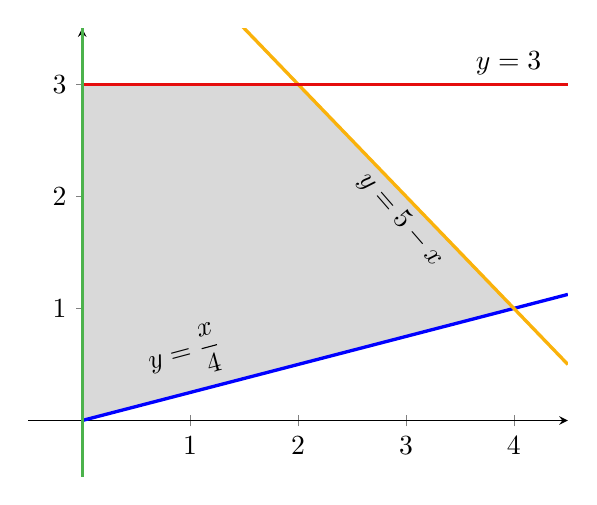
\begin{tikzpicture}
\begin{axis}[
axis lines=middle,
xmin=-0.5,xmax=4.5,ymin=-0.5,ymax=3.5
]
\addplot[very thick,blue, samples=300, domain=0:4.5, name path=A] {x/4}; 
\addplot[very thick,yellow!70!red, samples=300, domain=0:4.5, name path=B] {5-x}; 
\addplot[very thick,red!90!teal, samples=300, domain=0:4.5, name path=C] {3}; 
\addplot[very thick,green!70!magenta, samples=300, domain=0:4.5, name path=D] coordinates{(0,-6) (0,6)};
\addplot[gray!30] fill between[of=A and C,soft clip={domain=0:2}];
\addplot[gray!30] fill between[of=A and B,soft clip={domain=2:4}];
\node [rotate=15] at (axis cs:  0.95,  .59) {$\displaystyle y=\frac{x}{4}$};
\node [rotate=-49] at (axis cs:  2.95,  1.79) {$y=5-x$};
\node [rotate=0] at (axis cs:  3.95,  3.19) {$y=3$};
\end{axis}
\end{tikzpicture}

 \begin{parts}
\part[3] \label{part:one} One of the corner points of the feasible region is $(0,0)$. Find the other three corner points. Show Your work step by step and include explanations.
\fillwithdottedlines{3cm}


\part[2] Find the {\underline{maximum value}} of the objective function $10-4x+2y$ in the feasible region shown above. Please use the method described in class to solve this problem and show Your work step by step.
\fillwithdottedlines{3cm}

\part[2] Find the {\underline{point}}, in the feasible region shown above, where the objective function $10-4x+2y$ attains its minimum value. Please use the method described in class to solve this problem and show Your work step by step.
\fillwithdottedlines{3cm}
\end{parts}	

\bonusquestion[1]  True or False? {\emph{If a linear inequality in two unknowns $x$ and $y$ has a $\geq$ sign, then I will always need to shade above the line to get the solution set of the inequality.}} Explain Your reasoning (that is, if you think that the statement is always true, explain why; if You think that the statement is false, write an inequality for which the statement does not work.)
\fillwithdottedlines{3.5cm}

\newpage
%%%%%%%%%%%%%%%%%%%%%%%%%%%%%%
\question This question has\setcountertopartsofq{\arabic{question}}
\underline{\wordnum{numpofq}} (\arabic{numpofq}) parts
((a)---(\alph{numpofq})).

A fruit farm sells apples at a farm stand. Let $f(T)$ be the number of pounds of apples sold at the farm stand over $T$ days starting on September 1st, 2018 (so for example $f(3)$ is the sum of the number of pounds of apples sold on Sept 1st, 2nd and 3rd.) The revenue (in dollars) obtained by the farm from selling $A$ pounds of apples is given by the function $r(A)$. Assume that the functions $f(T)$ and $r(A)$ are one-to-one. 

\begin{parts}
	\part[2] What does $\displaystyle r^{-1}(200)$ represent in practical terms?
	\fillwithdottedlines{2cm}
\part[2] What does $\displaystyle r(f(4))$ represent in practical terms? \fillwithdottedlines{2cm}
\part[2] What does $\displaystyle f^{-1}(200)$ represent in practical terms?
\fillwithdottedlines{2cm}
	
	\end{parts}

\question This question has\setcountertopartsofq{\arabic{question}}
\underline{\wordnum{numpofq}} (\arabic{numpofq}) parts
((a)---(\alph{numpofq})).

Suppose the graph of the function $f$ is given. Describe how the graph of each function can be obtained from the graph of $f$.

\begin{parts}   
\part[1] $y = 5f(x + 9) - 6$

\begin{choices}
	\choice shift right 9 units, stretch horizontally by a factor of 5, then shift down 6 units
	\choice shift left 9 units, stretch vertically by a factor of 5, then shift down 6 units
\choice shift left 9 units, stretch horizontally by a factor of 5, then shift down 6 units
\choice shift left 9 units, stretch vertically by a factor of 5, then shift up 6 units    
\choice shift right 9 units, stretch horizontally by a factor of 5, then shift up 6 units
\end{choices}
    
\part[1] $y = 5f(x - 9) + 6$

\begin{choices}
	\choice shift left 9 units, stretch horizontally by a factor of 5, then shift up 6 units
	\choice shift right 9 units, stretch vertically by a factor of 5, then shift up 6 units
	\choice shift right 9 units, stretch horizontally by a factor of 5, then shift up 6 units
\choice shift right 9 units, stretch vertically by a factor of 5, then shift down 6 units    
 \choice left 9 units, stretch horizontally by a factor of 5, then shift down 6 units
\end{choices}
\end{parts}

\question[3] The following four transformations are applied to the function $\displaystyle f(x)=x^2$ to obtain a function $g(x)$.
\begin{enumerate}
	\item Vertical shift up 2 units, followed by:
	\item Horizontal shift 1 unit to the right, followed by:
	\item Vertical stretch by a factor of 2, followed by:
	\item Reflection around the $x$-axis.
\end{enumerate}

Write the final transformed function $g(x)$ as a quadratic function  in standard form, that is, $\displaystyle g(x)=a(x-h)^2+k$.  Show Your work step-by-step.
\fillwithdottedlines{2cm}
\newpage
\question This question has\setcountertopartsofq{\arabic{question}}
\underline{\wordnum{numpofq}} (\arabic{numpofq}) parts
((a)---(\alph{numpofq})).

A polynomial function $P(x)$  has exactly four distinct $x$ intercepts, $P(x)\to -\infty$ as $x\to-\infty$ and $P(x)\to \infty$ as $x\to \infty$.

\begin{parts}
	\part[2] Can $P$ have degree 6? Why? Why not?
\fillwithdottedlines{4cm}
	\part[2] Can $P$ have degree 5? Why? Why not?
	\fillwithdottedlines{4cm}
	\part[2] Does the polynomial $P$ have an inverse? Why? Why not?
	\fillwithdottedlines{4cm}		
	\end{parts}





\question This question has\setcountertopartsofq{\arabic{question}}
\underline{\wordnum{numpofq}} (\arabic{numpofq}) parts
((a)---(\alph{numpofq})).

The function $f(t)=4.5t+28$ gives the water level $f(t)$ (in feet) in a reservoir $t$ years after a dam was built.  

\begin{parts}
	\part[1] Which of the following statements best describes the meaning of the number 4.5  in practical terms?
	
	\begin{choices}
			\item  It is rise over run.
			\choice If we move 1 unit to the right, then we move 4.5 units up;
			\choice It is the change in $y$ over the change in $x$;
			\choice Every year, the water level changes by 4.5 feet;
			\choice Every year, the water level increases by 4.5 feet;
			%\item  It is rise over run.
	\end{choices}
	\part[1]  Describe the meaning of the number 28  in practical terms.
	
	\fillwithdottedlines{3cm}
\end{parts}
\newpage

\question This question has\setcountertopartsofq{\arabic{question}}
\underline{\wordnum{numpofq}} (\arabic{numpofq}) parts
((a)---(\alph{numpofq})).

The graph of a function $f(x)$ is shown below.



\begin{center}
	
	\begin{mfpic}[20]{-1}{6}{-1}{3}
		
		%\polyline{(0,-2), (4,1), (4,2), (5,3)}
		
		\polyline{(0,2), (1,2)} 
		
		\polyline{(1,1), (4,1)}
		
		\point[5pt]{(0,2), (1,2), (4,1)}
		\circle{(1,1),0.15}
		%\tlabel[cc](4,2.5){\scriptsize $(4,2)$}
		\axes
		
		\xmarks{1,2,3,4,5}
		
		\ymarks{-1,1,2,}
		
		\tlpointsep{4pt}
		
		\axislabels {x}{{\tiny $1$} 1, {\tiny $2$} 2, {\tiny $3$} 3, {\tiny $4$} 4,}
		
		\axislabels {y}{{\tiny $1$} 1,{\tiny $2$} 2,   {\tiny $-1$} -1}
		
		% Grid
		%\drawcolor[gray]{0.005}
		%\gridlines{1, 1}
		\drawcolor[gray]{0.95} 
		\grid{1,1}
		\tlabel[bl](-5,1){Graph of {\bf{f(x)}}}
	\end{mfpic}
	
\end{center}

\begin{parts}
	\part[1] Write the domain of $f$ in interval form. \dotfill
	\part[1] What is the range of $f$? \dotfill
	\part[2] Write the formula for $f$. (Note: $f$ is a piecewise-defined function.)
		\fillwithdottedlines{4cm}
	\part[4]  Fill out the table:
	
	\begin{minipage}{\linewidth}
		\centering
		
		{\setlength{\tabcolsep}{3.1em}  
			{\renewcommand{\arraystretch}{1.2}%
				
				\begin{tabular}{|l|l|l|l|l|}
					\hline
					$x$    & $0$ & $1$ & $2$ & $4$  \\ \hline
					$f(2x)$ &      &     &     &       \\ \hline
				\end{tabular}}} \quad
			\end{minipage}
			\smallskip
			
			%\part[2] Write the domain of $f(2x)$ in interval form. \dotfill
			%\part[2] Write the range of $f(2x)$ in interval form. \dotfill 
			\part[2]  The four  transformations listed below are applied (in the given order) to the function $f(x)$. On the grid provided below, draw the graph of the final transformed function $g(x)$ (that is, $g(x)$ is the outcome of applying the four transformations, in the given order, to the function $f(x)$ graphed above).
			
			\begin{minipage}[t][][b]{0.4\textwidth}
				%\begin{multicols}{2}
				
				\begin{enumerate}
					\item Horizontal shift left 1 units, followed by:
					
					\item  Reflection across the $y$-axis, followed by:
					
					\item  Vertical shift down 1 unit, followed by:
					
					\item Horizontal stretch by a factor of 2.
				\end{enumerate}
				
				%\end{multicols}
				%(Note: don't forget to draw and label the axes, and include units.)
			\end{minipage}
			\begin{minipage}[t][][b]{0.6\textwidth}
				\begin{center}
					
					
\begin{tikzpicture}
					\draw[gray!50, thin, step=0.5] (0,-2) grid (7,2);
					\end{tikzpicture}
				\end{center}
			\end{minipage}
			
			
			
			\bonuspart[2] Write the equation of the final transformed function $g(x)$. Show Your work step-by-step.   
			\fillwithdottedlines{4cm}
		\end{parts}
		
		\newpage
%%%%%%%%%%%%%%%%%%%%
\question This question has\setcountertopartsofq{\arabic{question}}
\underline{\wordnum{numpofq}} (\arabic{numpofq}) parts
((a)---(\alph{numpofq})).

  Are the statements listed below true or false? Give an explanation for Your answer (that is, if you think that the statement is always true, explain why; if you think that the statement is false, write an inequality for which the statement does not work.).
\begin{parts}
\part[2]  Every linear function $y=mx+b$ is one-to-one.

\fillwithdottedlines{2cm}

\part[2] The vertex of the parabola $f(x)=x^2+2x+1$ is $(1,0)$.

\fillwithdottedlines{2cm}


\part[2] The function $\displaystyle f(x)=\frac{(x-1)(x+1)}{(x+2)(x+1)}$ has exactly two vertical asymptotes, $x=-2$ and $x=-1$.

\fillwithdottedlines{2cm}

\part[2] The graph of a rational function cannot cross any of the vertical asymptotes.

\fillwithdottedlines{2cm}

\part[2] The rational function $\displaystyle f(x)=\frac{x^2+1}{x-3}$ has a slant asymptote.

\fillwithdottedlines{2cm}

\end{parts}
\bonusquestion[1] True or False? The range of the polynomial function $\displaystyle f(x)=2x^6+3x+4$ is all real numbers.
\begin{oneparchoices}
	\choice True \choice False
\end{oneparchoices}

\question This question has\setcountertopartsofq{\arabic{question}}
\underline{\wordnum{numpofq}} (\arabic{numpofq}) parts
((a)---(\alph{numpofq})). 

Consider the following functions.
$\displaystyle f(x) = \frac{2}{x-1},\,  g(x) = \frac{x}{x-1}$.

\begin{parts}
	\part[2] Find the domain of $f-g$ and write it in interval form. Show Your work step-by-step.
	\fillwithdottedlines{2cm}
	\part[2] Find the domain of $\displaystyle \frac{f}{g}$ and write it in interval form. Show Your work step-by-step.
	\fillwithdottedlines{2cm}	
\end{parts}

\newpage
%%%%%%%%%%%%%%%


\question This question has\setcountertopartsofq{\arabic{question}}
\underline{\wordnum{numpofq}} (\arabic{numpofq}) parts
((a)---(\alph{numpofq})). 

This problem is about the function $\displaystyle r(x)=\frac{(x-2)^2(x+2)}{(x-1)^2(x+1)}$.
\begin{parts}
	\vskip 0.2cm
	
	\part[2] The domain (in interval form) is \dotfill
		\vskip 0.2cm
		
	\part[2] Find the $x$ intercept(s).\dotfill
		\fillwithdottedlines{1cm}  %\hbox to 9cm{\hrulefill}
	\part[2] Find the $y$-intercept. \dotfill
		\fillwithdottedlines{1cm}
	\part[2] 	Write the equation(s) of  the vertical asymptote(s). 
	\fillwithdottedlines{1cm}
	\part[2] Write the equation of the horizontal asymptote and explain Your reasoning.
	\fillwithdottedlines{2cm}
	\bonuspart[2] 	On the grid provided below, draw a possible graph for $r(x)$. In order to receive any credit for this question, you must include {\bfseries{all}} of the following items:
	\begin{enumerate}
		\item Your graph includes units both on the $x$ and the $y$ axes.
		\item You have explained how You know the behavior of the function near the vertical asymptote(s). (Do the tails go in the same direction or in opposite direction? How do You know?)
		\item For each $x$ intercept, You have stated whether the graph goes across the $x$ axis or bounces off, and how You can see this from the equation.
	\end{enumerate}
	
		\fillwithdottedlines{4cm}
	
	
\begin{tikzpicture}
	\draw[gray!50, thin, step=0.5] (-7,-3) grid (7,4);
	\end{tikzpicture}	
	
\end{parts}

\newpage






\end{questions}
\newpage
\thispagestyle{empty}

\newpage
\thispagestyle{empty}
\setlength\fboxrule{2pt}\setlength\fboxsep{2mm}
\fbox{This page is intentionally left blank.} You may use it as scrap paper for your calculations.
\newpage
\thispagestyle{empty}

\newpage
\thispagestyle{empty}
\setlength\fboxrule{2pt}\setlength\fboxsep{2mm}
\fbox{This page is intentionally left blank.} You may use it as scrap paper for your calculations.
\newpage
\thispagestyle{empty}

\newpage
\thispagestyle{empty}
\setlength\fboxrule{2pt}\setlength\fboxsep{2mm}
\fbox{This page is intentionally left blank.} You may use it as scrap paper for your calculations.
\end{document}                 